\chapter{Исследовательский раздел}

В данном разделе приведены технические характеристики устройства, на котором проводилось измерение времени работы программного обеспечения, а также результаты замеров времени работы программы.

Целью исследования является провести анализ скорости работы алгоритма морфинга изображений с использованием алгоритма Z-буфера для визуализации.

\section{Технические характеристики}

Технические характеристики устройства, на котором выполнялось тестирование:
\begin{enumerate}
	\item Процессор Intel(R) Core(TM) i7-11700K @ 3.60МГц.
	\item Оперативная память - 32 GB.
\end{enumerate}

Во время тестирования программа была запущена на виртуальной машине Ubuntu 22.04 из операционной системы Windows 10. 
Технические характеристики виртуальной машины:
\begin{enumerate}
	\item Число ядер - 4.
	\item Оперативная память - 20.9 GB.
\end{enumerate}

\section{Результаты исследования}

Для исследования зависимости времени от размеров фигуры использовались фигуры с различным числом вершин и ребер. 
На графиках учитываются вершины и ребра результирующих фигур, так как до начала морфинга каждая фигура достраивается либо разрушается так, чтобы количество вершин и ребер стало таким же, как у фигуры, к которой она будет преобразована.
 
Для каждого случая было проведено по 10 тестов, выбрано среднее значение по времени. 
Результаты исследования представлены на рисунках~\ref{fig:res_tests_vertices.pdf} - \ref{fig:res_tests_edges.pdf} и в таблице~\ref{tbl:time_measurements}.

\begin{table}[H]
	\begin{center}
		\begin{threeparttable}
			\captionsetup{justification=raggedright,singlelinecheck=off}
			\caption{Результаты исследования}
			\label{tbl:time_measurements}
			\begin{tabular}{|r|r|r|}
				\hline
				Кол-во вершин & Кол-во ребер & Время (мс) \\
				\hline
				8 & 24 &$ 1 $\\
				\hline
				281 & 1 124 &$ 1 $\\ 
				\hline
				1 136 & 6 246 &$ 2 $\\
				\hline
				2 210 & 8 568 &$ 4 $\\
				\hline
				5 530 & 21 712 &$ 8 $\\
				\hline
				7 338 & 29 344 &$ 10 $\\
				\hline
				10 194 & 40 772 &$ 17 $\\
				\hline
				25 075 & 91 680 &$ 30 $\\
				\hline
				35 986 & 143 936 &$ 53 $\\
				\hline
				40 062 & 161 472 &$ 56 $\\
				\hline
			\end{tabular}
		\end{threeparttable}
	\end{center}
\end{table}

\begin{figure}[h]
	\centering
	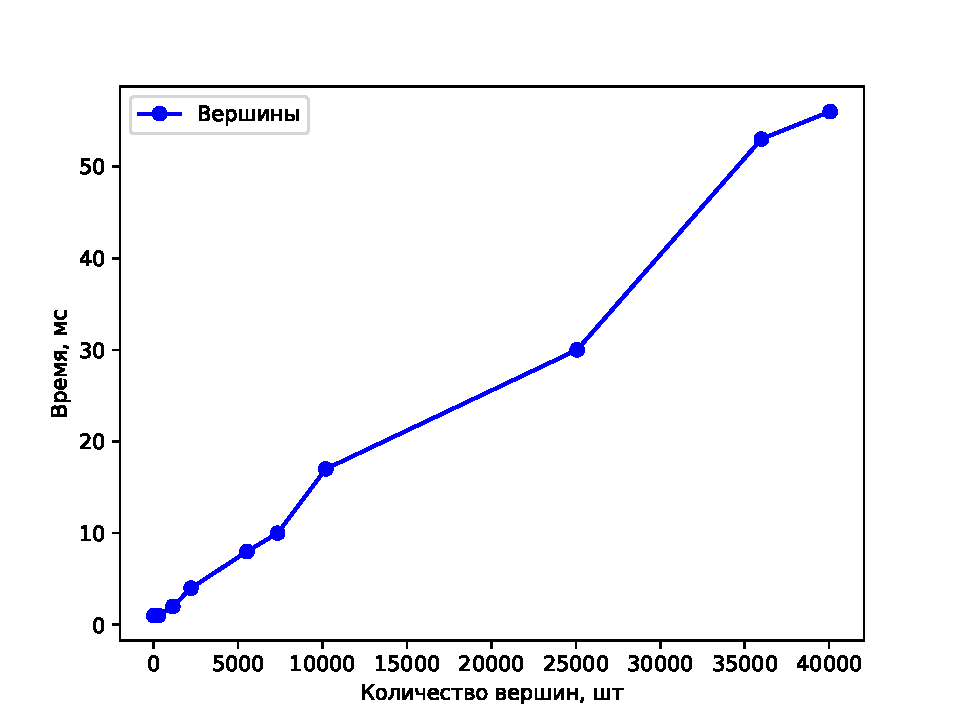
\includegraphics{images/tests_vertices.pdf}
	\caption{Результаты исследования}
	\label{fig:res_tests_vertices.pdf}
\end{figure}

\begin{figure}[h]
	\centering
	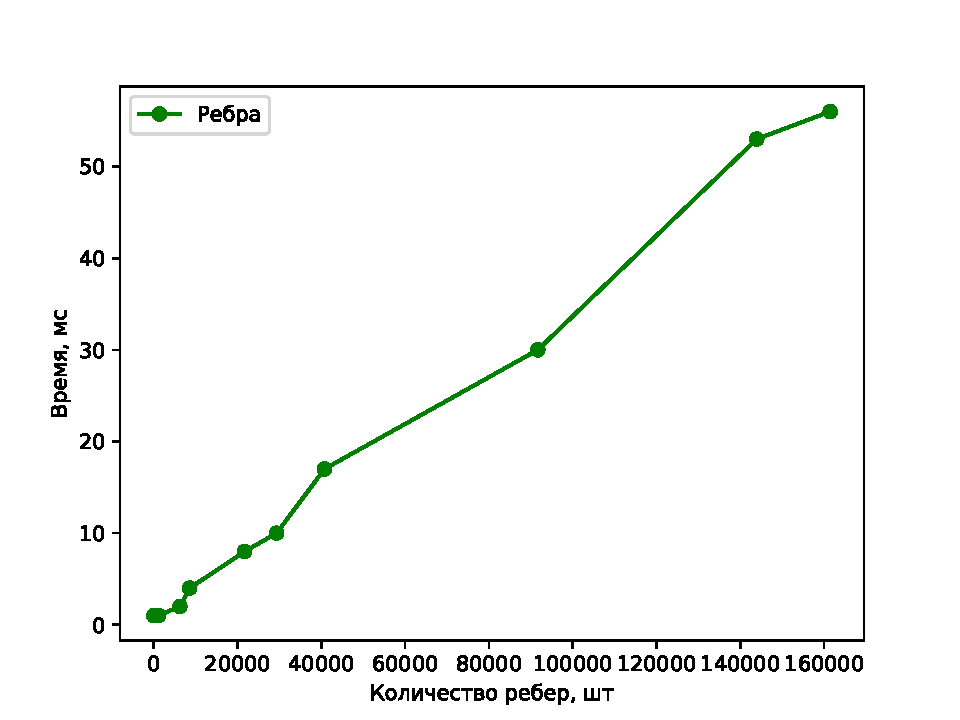
\includegraphics{images/tests_edges.pdf}
	\caption{Результаты исследования}
	\label{fig:res_tests_edges.pdf}
\end{figure}

\newpage

Из проведенного исследования можно сделать вывод, что время визуализации сцены во время морфинга линейно зависит от количества вершин и ребер результирующей фигуры.

\section*{Выводы из исследовательского раздела}

В данном разделе приведены результаты работы программного обеспечения и проведено исследование, показывающее зависимость времени визуализации сцены во время морфинга от количества вершин и ребер результирующей фигуры.

Результаты исследования совпали с ожидаемыми, так как в ходе исследования было установлено, что время работы увеличивается с увеличением количества вершин и ребер у объекта.
